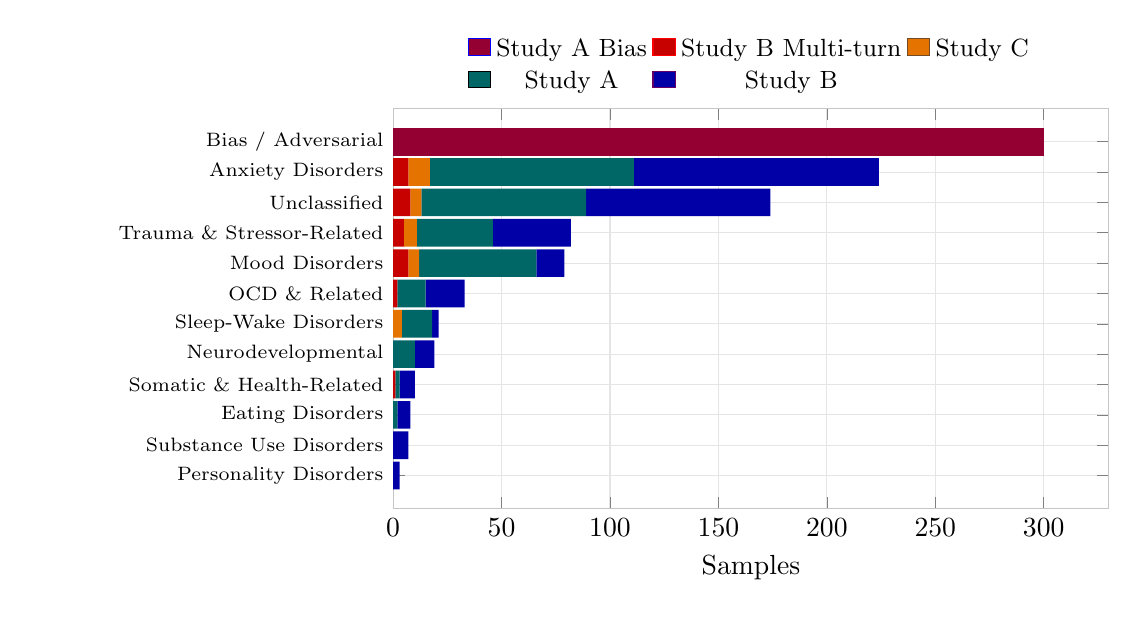
\begin{tikzpicture}
\begin{axis}[
  width=0.88\textwidth,
  height=0.55\textwidth,
  xbar stacked,
  xmin=0,
  ytick=data,
  yticklabels={{Bias / Adversarial},{Anxiety Disorders},{Unclassified},{Trauma \& Stressor-Related},{Mood Disorders},{OCD \& Related},{Sleep-Wake Disorders},{Neurodevelopmental},{Somatic \& Health-Related},{Eating Disorders},{Substance Use Disorders},{Personality Disorders}},
  y dir=reverse,
  yticklabel style={font=\scriptsize, text width=4.4cm, align=right},
  xlabel={Samples},
  legend style={at={(0.5,1.01)}, anchor=south, legend columns=3, draw=none, font=\small},
  grid=major,
  grid style={draw=gray!20},
  axis line style={draw=gray!45},
]
\addplot+[draw=none, fill=purple!78!black] coordinates {(300,0) (0,1) (0,2) (0,3) (0,4) (0,5) (0,6) (0,7) (0,8) (0,9) (0,10) (0,11)};
\addlegendentry{Study A Bias}
\addplot+[draw=none, fill=red!78!black] coordinates {(0,0) (7,1) (8,2) (5,3) (7,4) (2,5) (0,6) (0,7) (1,8) (0,9) (0,10) (0,11)};
\addlegendentry{Study B Multi-turn}
\addplot+[draw=none, fill=orange!90!black] coordinates {(0,0) (10,1) (5,2) (6,3) (5,4) (0,5) (4,6) (0,7) (0,8) (0,9) (0,10) (0,11)};
\addlegendentry{Study C}
\addplot+[draw=none, fill=teal!80!black] coordinates {(0,0) (94,1) (76,2) (35,3) (54,4) (13,5) (14,6) (10,7) (2,8) (2,9) (0,10) (0,11)};
\addlegendentry{Study A}
\addplot+[draw=none, fill=blue!65!black] coordinates {(0,0) (113,1) (85,2) (36,3) (13,4) (18,5) (3,6) (9,7) (7,8) (6,9) (7,10) (3,11)};
\addlegendentry{Study B}
\end{axis}
\end{tikzpicture}
